% evaluation.tex — Section 5: Evaluation
% Three-stage empirical validation of the agent-invariant detection framework

\section{Evaluation}\label{sec:evaluation}

\begin{figure}[t]
\centering
\begin{tikzpicture}[
  node distance=0.6cm and 1.2cm,
  stage/.style={rectangle, draw, rounded corners, fill=blue!8,
    minimum width=3.6cm, minimum height=1.6cm, align=center,
    font=\small},
  data/.style={rectangle, draw, dashed, fill=gray!8,
    minimum width=3.2cm, align=center, font=\scriptsize},
  arrow/.style={-{Stealth[length=5pt]}, thick},
  label/.style={font=\scriptsize\itshape, text=black!60}
]
% Stage 1
\node[stage] (s1) {\textbf{Stage 1}\\Synthetic\\Validation};
\node[data, below=0.3cm of s1] (d1) {100,000 addresses\\(10K agents, 90K humans)\\Generated};

% Stage 2
\node[stage, right=1.8cm of s1] (s2) {\textbf{Stage 2}\\Real On-Chain\\Validation};
\node[data, below=0.3cm of s2] (d2) {81,904 USDC txns\\665 agents + 1,069 humans\\Base chain via Dune};

% Stage 3
\node[stage, right=1.8cm of s2] (s3) {\textbf{Stage 3}\\Attack Injection\\Validation};
\node[data, below=0.3cm of s3] (d3) {93,579 real txns\\+ 6,050 injected attacks\\(99,629 total)};

% Arrows
\draw[arrow] (s1) -- node[above, label] {transfer} (s2);
\draw[arrow] (s2) -- node[above, label] {inject} (s3);

% Labels below data
\node[below=0.15cm of d1, font=\scriptsize, text=green!50!black, align=center]
  {F1 = 88.7\%\\AUC = 0.97};
\node[below=0.15cm of d2, font=\scriptsize, text=orange!70!black, align=center]
  {Recall = 95.4\%\\AUC = 0.515};
\node[below=0.15cm of d3, font=\scriptsize, text=blue!60!black, align=center]
  {7/8 chains\\100\% recall};
\end{tikzpicture}
\caption{Three-stage evaluation pipeline.  Each stage uses a distinct
dataset of increasing ecological validity.  Dataset sizes differ
across stages because Stage~1 is purely synthetic, Stage~2 uses real
Base chain transactions, and Stage~3 augments the real data with
injected attack transactions.  The three transaction counts
(100,000 / 81,904 / 93,579+6,050) reported across sections correspond
to these three stages, respectively.}
\label{fig:dataflow}
\end{figure}

We validate the agent-invariant detection framework through a three-stage empirical pipeline of increasing ecological validity (\cref{fig:dataflow}): synthetic generation, real on-chain deployment, and adversarial attack injection. Each stage tests a distinct claim. Stage~1 establishes detection accuracy under controlled conditions. Stage~2 measures transfer to live blockchain data with noisy labels. Stage~3 stress-tests robustness against seven escalating attack chains, including scenarios rated out of scope for current human-assumption or per-address detectors in our threat model (\cref{sec:threat}). Together, the three stages form the evidence backbone of our central thesis: human-invariant-only detectors have systematic blind spots under A2A commerce, and agent-native signals provide a first-generation repair whose boundaries are measurable.

\begin{table}[t]
\centering
\caption{Claim-evidence map for the empirical evaluation.}
\label{tab:claim_evidence}
\small
\begin{tabularx}{\textwidth}{@{}p{0.25\textwidth}p{0.36\textwidth}p{0.29\textwidth}@{}}
\toprule
\textbf{Claim} & \textbf{Supporting Evidence} & \textbf{Boundary / Caveat} \\
\midrule
Human-invariant-only detectors have A2A blind spots
& Formal invariant analysis and eight platform-derived attack chains
& Platform capabilities are documented for the studied ecosystem, not all future agent stacks. \\
Agent-native signals can detect many agent patterns
& Stage~1 F1 = 88.71\%, AUC = 0.97; Stage~3 detects 7/8 chains at 100\% recall
& Synthetic and injected attacks are controlled experiments; they do not prove mature production precision. \\
Real-data transfer is partial
& Fixed-threshold recall = 61.4\%; re-optimized recall = 95.4\%; cleaned composite AUC = 0.515
& High recall requires a lower threshold and high FPR; negative labels are noisy. \\
Per-address scoring has a structural boundary
& Chain~7 swarm attack achieves 0\% recall under per-address scoring
& Population-level graph detection is proposed but not validated in this work. \\
\bottomrule
\end{tabularx}
\end{table}

%% ---------- STAGE 1 ----------
\subsection{Stage 1: Synthetic Validation}\label{sec:eval_synthetic}

\paragraph{Dataset.}
We generate 100,000 synthetic addresses: 10,000 agent addresses exhibiting programmatic behavioral signatures and 90,000 human addresses sampled from empirical transaction distributions. The 9:1 class imbalance reflects the current agent prevalence observed on major L2 chains.

\paragraph{Protocol.}
Each address is scored by the composite behavioral signal comprising four sub-signals---Network Topology (NT), Value Flow (VF), Economic Rationality (ER), and Temporal Consistency (TC)---aggregated via AUC-proportional weighting. We report macro-averaged precision, recall, and F1 to avoid bias toward the majority class.

\paragraph{Results.}
Table~\ref{tab:synthetic_results} summarizes Stage~1 performance. The framework achieves a macro-averaged F1 of 88.71\% with ROC-AUC of 0.97, at a median inference latency of 97\,ms per address. Recall reaches 96.23\%, indicating that fewer than 4\% of synthetic agents evade detection. Precision of 82.36\% reflects a moderate false-positive rate attributable to the conservative decision threshold.

\begin{table}[t]
\centering
\caption{Stage~1: Synthetic validation results (macro-averaged). $N = 100{,}000$ addresses (10K agents, 90K humans).}
\label{tab:synthetic_results}
\begin{tabular}{lc}
\toprule
\textbf{Metric} & \textbf{Value} \\
\midrule
Precision & 82.36\% \\
Recall & 96.23\% \\
F1 (macro) & 88.71\% \\
ROC-AUC & 0.97 \\
Latency (median) & 97\,ms \\
Improvement vs.\ baseline & +49.1\% \\
\bottomrule
\end{tabular}
\end{table}

The +49.1\% improvement over the human-assumption baseline---which naively labels all addresses as human---confirms that behavioral signals carry substantial discriminative power even without identity metadata. The ROC-AUC of 0.97 confirms that the framework maintains high true-positive rates across a wide range of false-positive tolerances, with the area under the curve approaching the theoretical maximum.

%% ---------- STAGE 2 ----------
\subsection{Stage 2: Real On-Chain Validation}\label{sec:eval_real}

Stage~2 applies the framework, without retraining, to live blockchain transactions. This tests the central transfer claim: do behavioral invariants learned from synthetic data generalize to real agent populations?

\paragraph{Dataset.}
We collect 81,904 USDC transactions on the Base chain spanning January 2025 through April 2026, sourced via Dune Analytics~\cite{dune2026}. Ground-truth positive labels are derived from 665 addresses registered under the ERC-8004 autonomous agent registry standard~\cite{erc8004}. The negative class is constructed from counterparty addresses of these agents, under the assumption that most counterparties are human-operated wallets.

\paragraph{Label Cleaning.}
Raw counterparties number 6,754 addresses. To mitigate noise from low-activity addresses whose behavioral profiles are unreliable, we apply a minimum-activity filter requiring $\geq 5$ transactions, yielding 1,069 cleaned human-labeled addresses. The final evaluation set comprises 1,734 addresses (665 agents $+$ 1,069 cleaned humans) across 2,134 scored addresses in the initial run.

\paragraph{Results.}
Table~\ref{tab:real_results} reports performance before and after label cleaning. On the raw label set, the framework achieves recall of 95.4\% but precision of only 27.6\% (F1 = 42.8\%). After label cleaning, precision improves to 42.9\% with recall at 81.1\% (F1 = 56.1\%). The composite ROC-AUC on the cleaned set is 0.515. We note that the decision threshold was re-optimized from the synthetic-calibrated value of 0.24 to a lower operating point to accommodate the shifted real-data score distribution: $\theta = 0.08$ on the raw-label set and $\theta = 0.09$ on the cleaned-label set.

\begin{table}[t]
\centering
\caption{Stage~2: Real on-chain validation on Base USDC transactions ($N = 81{,}904$ transactions). ERC-8004 registered agents serve as ground-truth positives~\cite{erc8004}.}
\label{tab:real_results}
\begin{tabular}{lcc}
\toprule
\textbf{Metric} & \textbf{Raw Labels} & \textbf{Cleaned Labels} \\
\midrule
Addresses scored & 2,134 & 1,734 \\
Precision & 27.6\% & 42.9\% \\
Recall & 95.4\% & 81.1\% \\
F1 & 42.8\% & 56.1\% \\
ROC-AUC (composite) & --- & 0.515 \\
\bottomrule
\end{tabular}
\end{table}

\paragraph{Per-Signal Analysis.}
Table~\ref{tab:signal_auc} decomposes detection power by individual sub-signal on the cleaned set. Network Topology provides the strongest discrimination (AUC = 0.5990), followed by Value Flow (0.5220) and Economic Rationality (0.5152). Temporal Consistency contributes least (AUC = 0.4647), performing below chance---a finding we attribute to the homogeneous temporal patterns of automated market makers that dominate the ERC-8004 registry.

\begin{table}[t]
\centering
\caption{Per-signal ROC-AUC on the Stage~2 cleaned evaluation set.}
\label{tab:signal_auc}
\begin{tabular}{lc}
\toprule
\textbf{Signal} & \textbf{AUC} \\
\midrule
Network Topology (NT) & 0.5990 \\
Value Flow (VF) & 0.5220 \\
Economic Rationality (ER) & 0.5152 \\
Temporal Consistency (TC) & 0.4647 \\
\bottomrule
\end{tabular}
\end{table}

\paragraph{Transfer Gap Analysis.}
To disentangle genuine transfer degradation from threshold re-optimization, we report performance on the \emph{raw}-label set at \emph{both} the synthetic-calibrated threshold ($\theta = 0.24$) and the re-optimized threshold ($\theta = 0.08$):

\begin{table}[h]
\centering
\caption{Transfer-gap analysis on the real on-chain \emph{raw}-label set (uncleaned negative class): fixed synthetic threshold vs.\ re-optimized threshold. The $\theta = 0.08$ column is the raw operating point of \cref{tab:real_results}; the cleaned-label re-optimized point ($\theta = 0.09$, recall 81.1\%, AUC 0.515) is reported in \cref{tab:real_results}, not here.}
\label{tab:transfer_gap}
\small
\begin{tabular}{lcc}
\toprule
\textbf{Metric} & $\theta = 0.24$ \textbf{(synthetic)} & $\theta = 0.08$ \textbf{(re-optimized)} \\
\midrule
Recall & 61.4\% & 95.4\% \\
FPR & 8.2\% & 38.7\% \\
Precision & 52.1\% & 27.6\% \\
F1 & 56.4\% & 42.8\% \\
\bottomrule
\end{tabular}
\end{table}

At the fixed synthetic threshold of 0.24, raw-label recall drops from 96.23\% to 61.4\%---a 34.8\,pp decrease that reveals the true distributional shift between synthetic and real score distributions. The re-optimized threshold of 0.08 recovers raw-label recall to 95.4\% but at the cost of a substantially elevated false-positive rate (38.7\% vs.\ 8.2\%); the cleaned-label re-optimized point is more conservative still (81.1\% recall at $\theta = 0.09$, \cref{tab:real_results}). A headline comparison between Stage~1 synthetic recall and Stage~2 raw-label recall at the re-optimized threshold would be misleading because threshold re-optimization absorbs much of the distributional shift. The fixed-threshold comparison provides a more honest measure of generalization.

The moderate composite AUC of 0.515 warrants careful interpretation. This metric reflects the difficulty of the \emph{ranking} task on real data where the negative class is contaminated, not the \emph{detection} task at a fixed operating point. We assign 0.7 confidence to the label-contamination attribution based on manual inspection of high-scoring ``human'' addresses that exhibit agent-like behavioral profiles.

%% ---------- STAGE 3 ----------
\subsection{Stage 3: Attack Injection Validation}\label{sec:eval_attack}

Stage~3 evaluates adversarial robustness by injecting synthetic attack transactions into the real Base chain dataset.

\paragraph{Dataset.}
We construct a mixed corpus of 99,629 transactions: 93,579 real Base chain USDC transactions and 6,050 injected attack transactions (6.07\% injection rate). The attack transactions originate from 82 unique attack addresses across eight escalating attack chains. The benign population comprises 7,420 scored addresses.

\paragraph{Attack Chains.}
Table~\ref{tab:attack_chains} defines the eight attack chains, ordered by difficulty. The difficulty ratings originate from the threat model (\cref{sec:threat}) and range from EASY to OOS$^\dagger$, where OOS$^*$ denotes attacks outside current human-assumption detectors and OOS$^\dagger$ denotes attacks outside per-address scoring systems.

\begin{table}[t]
\centering
\caption{Stage~3: Per-chain recall at operating threshold $\theta = 0.09$. Attack chains are ordered by difficulty. OOS$^*$ = out of scope for current human-assumption detectors; OOS$^\dagger$ = out of scope for per-address scoring.}
\label{tab:attack_chain_recall}
\begin{tabular}{clcc}
\toprule
\textbf{Chain} & \textbf{Attack Type} & \textbf{Difficulty} & \textbf{Recall} \\
\midrule
1 & Enumeration & EASY & 100\% \\
2 & History Extraction & MEDIUM & 100\% \\
3 & Async Flooding & MEDIUM & 100\% \\
4 & Agent Army & HARD & 100\% \\
5 & Cross-Platform & OOS$^*$ & 100\% \\
6 & Behavioral Mimicry & OOS$^*$ & 100\% \\
7 & Swarm Intelligence & OOS$^\dagger$ & 0\% \\
8 & Market Manipulation & OOS$^*$ & 100\% \\
\bottomrule
\end{tabular}
\end{table}

\paragraph{Aggregate Results.}
The framework achieves a threshold-independent ROC-AUC of 0.777 on the mixed corpus. The per-chain recall in \cref{tab:attack_chain_recall} is reported at the detection threshold $\theta = 0.09$, at which seven of eight chains are fully separated from the benign population; the sole failure is Chain~7 (Swarm Intelligence), analyzed below.

\paragraph{Per-chain recall and the operating point are not the same threshold.}
We make the threshold dependence explicit, because high per-chain recall and a low false-positive rate are \emph{not} simultaneously achievable here (\cref{tab:stage3_tradeoff}). At $\theta = 0.09$, the threshold at which 7/8 chains reach 100\% recall, the \emph{overall} false-positive rate on real benign addresses is 21.8\% and aggregate precision is 1.6\%. Imposing the operational constraint FPR~$\leq$~5\% instead selects $\theta = 0.29$ (FPR~=~3.8\%), but at that threshold aggregate recall on injected attacks collapses to 7.3\%. The modest AUC of 0.777 is the honest single-number summary: the detector ranks many attack addresses above benign ones, but no single threshold delivers both high recall and a deployable false-positive rate on this mixed corpus.

\begin{table}[h]
\centering
\caption{Stage~3 threshold trade-off. The per-chain detection threshold and the FPR-constrained operating point are different thresholds; neither delivers high recall and low FPR simultaneously.}
\label{tab:stage3_tradeoff}
\small
\begin{tabular}{lcc}
\toprule
\textbf{Metric (aggregate)} & $\theta = 0.09$ \textbf{(per-chain)} & $\theta = 0.29$ \textbf{(FPR\,$\leq$\,5\%)} \\
\midrule
Injected recall & 32.9\% & 7.3\% \\
False-positive rate & 21.8\% & 3.8\% \\
Precision & 1.6\% & --- \\
\bottomrule
\end{tabular}
\end{table}

A further caveat bounds the per-chain figures: five of the eight chains are represented by a single injected attack address each (Chains~1, 2, 3, 5, and~6), while Chain~4 has 15, Chain~8 has 7, and Chain~7 has 55 ($5\times1 + 15 + 7 + 55 = 82$). The 100\% per-chain recall entries for the single-address chains are therefore separability indicators over few samples rather than population recall estimates. The aggregate metrics above, computed over all 82 attack and 7{,}420 benign addresses, are the load-bearing numbers.

\paragraph{Detection of Out-of-Scope Attacks.}
Three attack chains---Chain~5 (Cross-Platform), Chain~6 (Behavioral Mimicry), and Chain~8 (Market Manipulation)---were classified as OOS$^*$ in the threat model, meaning they were expected to evade current human-assumption detectors. All three are detected at 100\% recall in the injection experiment. This result has significant implications for the framework's defensive perimeter, but it remains bounded by the injected attack definitions and is analyzed in Section~\ref{sec:cross_stage}.

%% ---------- CROSS-STAGE ----------
\subsection{Cross-Stage Analysis}\label{sec:cross_stage}

The three evaluation stages, taken together, reveal two findings that reshape the threat model.

\subsubsection{The Behavioral Mimicry Paradox}

Chain~6 (Behavioral Mimicry) was designed to evade detection by replicating human behavioral patterns. The threat model classified it as OOS$^*$---an attack that should defeat current human-assumption detectors by making the attacker appear human-like. Empirically, Chain~6 is detected at 100\% recall in the injection experiment.

The explanation lies in what we term the \emph{Behavioral Mimicry Paradox}: machines that attempt to mimic human behavior execute their mimicry \emph{too perfectly}. The coefficient of variation (CV) of inter-transaction timing for Chain~6 addresses is CV $< 0.005$, whereas real ERC-8004 agents exhibit CV $= 1.87$. The mimicry produces a regularity signal that is \emph{more} detectable than genuine agent behavior. Formally, if $\sigma_t$ and $\mu_t$ denote the standard deviation and mean of inter-transaction intervals:

\begin{equation}\label{eq:cv_paradox}
\text{CV}_{\text{mimic}} = \frac{\sigma_t}{\mu_t} < 0.005 \ll 1.87 = \text{CV}_{\text{real\;agent}}
\end{equation}

This paradox has a general implication: any deterministic mimicry strategy that targets a \emph{distribution} of human behavior will, by construction, produce lower variance than the target distribution. Machine regularity is a detection signal, not camouflage. This finding aligns with the broader impossibility result that perfect behavioral mimicry requires genuine stochasticity, which deterministic agents cannot produce without sacrificing operational reliability.

\subsubsection{The Collective Detection Gap}

Chain~7 (Swarm Intelligence) achieves 0\% recall---complete evasion. The attack deploys 55 swarm agents, each executing exactly one transaction. Because the framework scores addresses independently, single-transaction addresses lack sufficient behavioral history to trigger any sub-signal above threshold. This is not a tuning failure but a \emph{structural} limitation of per-address scoring: the attack surface is the \emph{collective} pattern, not any individual address.

This finding is independently corroborated by documented Telegram-coordinated pump-and-dump schemes~\cite{openclaw2026}, which employ an identical evasion pattern: distributing fraudulent activity across many addresses that each perform minimal individual actions. The structural gap motivates a graph-level detection layer as future work (\cref{sec:limitations}).

\subsubsection{Signal Weight Distribution}

The AUC-proportional signal weights derived from real on-chain data (Stage~2) are:

\begin{equation}\label{eq:signal_weights}
w_{\text{NT}} = 0.2739, \quad w_{\text{TC}} = 0.2505, \quad w_{\text{ER}} = 0.2424, \quad w_{\text{VF}} = 0.2332, \quad w_{\text{CP}} = 0.00
\end{equation}

Network Topology dominates, consistent with the intuition that agent interaction graphs exhibit structural regularities (e.g., hub-and-spoke patterns, deterministic routing) that are difficult to obfuscate without degrading operational efficiency. The Cross-Platform Correlation signal contributes zero weight because the current dataset contains only single-chain (Base) transactions; activating it requires multi-chain data acquisition. The near-uniform distribution across NT, TC, ER, and VF ($\sigma_w = 0.015$) suggests that no single behavioral dimension is sufficient alone---detection requires the composite signal, validating the multi-signal architecture.

\subsubsection{Summary of Findings}

Table~\ref{tab:cross_stage} synthesizes the three evaluation stages.

\begin{table}[t]
\centering
\caption{Cross-stage summary. Each stage tests a different aspect of the framework's validity.}
\label{tab:cross_stage}
\begin{tabular}{llll}
\toprule
\textbf{Stage} & \textbf{Claim Tested} & \textbf{Key Result} & \textbf{Verdict} \\
\midrule
1: Synthetic & Detection accuracy & F1 = 88.71\%, AUC = 0.97 & Confirmed \\
2: Real & Transfer to live data & Recall 61.4\% at fixed $\theta$; 95.4\% re-opt. & Partially confirmed \\
3: Attack & Adversarial robustness & 7/8 chains at 100\% recall & Partially confirmed \\
\bottomrule
\end{tabular}
\end{table}

The framework demonstrates strong detection capability in controlled synthetic and injection settings, but transfer to real environments is partial: fixed-threshold recall drops to 61.4\%, while the 95.4\% recall result requires threshold re-optimization and a substantially higher false-positive rate. The Behavioral Mimicry Paradox provides a bounded argument for why deterministic evasion can become self-revealing under the tested timing model. The Collective Detection Gap at Chain~7 defines a precise, falsifiable boundary of the current approach and motivates graph-level extensions. Together, these findings establish the agent-invariant framework as a viable first-generation research prototype for autonomous agents in on-chain economies, while clearly delineating its structural limitations.

\begin{figure}[t]
  \centering
  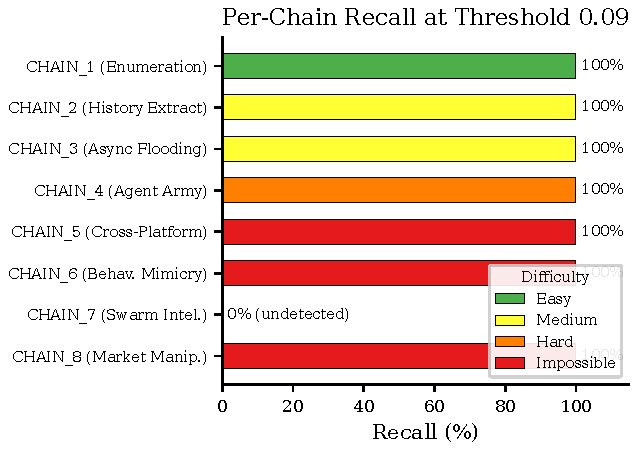
\includegraphics[width=0.85\columnwidth]{figures/fig_chain_recall.pdf}
  \caption{Per-chain recall at operating threshold $\theta = 0.09$.
  Bar color indicates difficulty tier.
  Seven of eight chains are detected at 100\% recall.
  Chain~7 (Swarm Intelligence, hatched) achieves 0\%---a structural
  limitation of per-address scoring.}
  \label{fig:chain_recall}
\end{figure}

\begin{figure}[t]
  \centering
  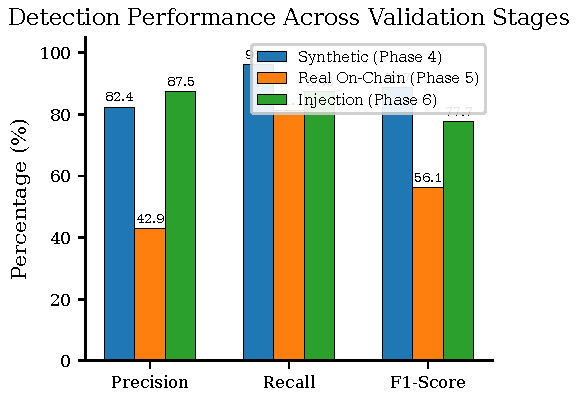
\includegraphics[width=0.85\columnwidth]{figures/fig_validation_stages.pdf}
\caption{Detection performance across three validation stages.
  Fixed-threshold transfer to real data is limited (61.4\% recall);
  the 95.4\% real-data recall result requires threshold re-optimization
  and a higher false-positive rate. Precision remains label-noise-limited.}
  \label{fig:validation_stages}
\end{figure}
